\documentclass[a4paper,german,12pt,smallheadings]{scrartcl}
\usepackage[T1]{fontenc}
\usepackage[utf8]{inputenc}
\usepackage{babel}
\usepackage{geometry}
\usepackage{tikz}
\usepackage{wrapfig}
\usepackage[fleqn]{amsmath}
\usepackage{amssymb}
\usepackage{float}
\usepackage{enumerate}
\usepackage{listings} % Source code
\usepackage{lscape} % landscape
\usepackage{commath} % http://tex.stackexchange.com/questions/14821/whats-the-proper-way-to-typeset-a-differential-operator
\usepackage{cancel}
\usepackage[fleqn]{mathtools}
% Number only referenced equations
%\mathtoolsset{showonlyrefs}

%\usepackage{wrapfig}
\usepackage{siunitx}
\sisetup{separate-uncertainty=true,locale=DE}

% New command for color underlining
\usepackage{xcolor}
\newcommand\invisiblesection[1]{%
    \refstepcounter{section}%
      \addcontentsline{toc}{section}{\protect\numberline{\thesection}#1}%
        \sectionmark{#1}}
\newsavebox\MBox
\newcommand\colul[2][red]{{\sbox\MBox{$#2$}%
  \rlap{\usebox\MBox}\color{#1}\rule[-1.2\dp\MBox]{\wd\MBox}{0.5pt}}}

\restylefloat{table}
\geometry{a4paper, top=15mm, left=20mm, right=10mm, bottom=20mm, headsep=10mm, footskip=12mm}
\linespread{1.5}
\setlength\parindent{0pt}
\DeclareMathOperator{\Tr}{Tr}
\DeclareMathOperator{\Var}{Var}
\begin{document}

\begin{titlepage}
\newcommand{\HRule}{\rule{\linewidth}{0.5mm}}

\begin{center}
  \textsc{\Large Physikalisches Grundpraktkum 1}
  \HRule\\[0.4 cm]
  {\huge \bfseries Gleichmäßig beschleunigte Drehbewegungen}
  \HRule\\[0.4 cm]

  \begin{minipage}{0.65\textwidth}
  \begin{flushleft}
    Markus Fenske \texttt{<iblue@zedat.fu-berlin.de>} \\
    Paul Rahmann \texttt{<paulrahmann@zedat.fu-berlin.de>}
  \end{flushleft}
  \end{minipage}
  \hfill
  \begin{minipage}{0.30\textwidth}
  \begin{flushright}
    Tutor: Christian Hindermann \\
    Versuchstag: 6. Juni 2014
  \end{flushright}
  \end{minipage}

  \vspace{1cm}

  \tableofcontents


  %{\large \today}
  \vfill
\end{center}
\newpage

\end{titlepage}

\allowdisplaybreaks % Seitenumbrüche in Formeln erlauben
\begin{center}
\bfseries % Fettdruck einschalten
\sffamily % Serifenlose Schrift
\vspace{-40pt}
Physikalisches Grundpraktikum 1, Sommersemester 2014

Markus Fenske \texttt{<iblue@zedat.fu-berlin.de>}

Paul Rahmann \texttt{<paulrahmann@zedat.fu-berlin.de>}

Harmonische Schwingungen, Tutor: Boden
\vspace{-10pt}
\end{center}

\section{Physikalische Grundlagen}
Der harmonische Oszillator ist ein System, das bei Auslenkung aus der Ruhelage
eine lineare Rückstellkraft erfährt. Zusätzlich kann noch eine
geschwindigkeitsabhängige Reibungskraft angenommen werden, so dass aus der
Grundgleichung der Mechanik $F=ma$ das Bewegungsgesetz folgt:
\begin{equation}
  m \ddot{x} + k \dot{x} + D x = 0
\end{equation}

Dabei ist $m$ die Masse des Schwingers, $k$ die Reibungskonstante, $D$ die
Federkonstante und $x(t)$ die Auslenkung. Der reibungsfreie Fall ist enthalten,
wenn man $k=0$ setzt.

Mit den Kürzungen
\begin{equation}
  \delta = \frac{k}{2m}
  \label{eq:delta}
\end{equation}

\begin{equation}
  \omega = \sqrt{\frac{D}{m} - \frac{k^2}{4m^2}}
  \label{eq:omega}
\end{equation}

ist die Lösung
\begin{equation}
  x(t) = C_1 e^{- \delta t} e^{i \omega t} + C_2 e^{-\delta t} e^{-i \omega t}
  \label{eq:x_t}
\end{equation}

\subsection{Schwingfall, Kriechfall, Aperiodischer Grenzfall}
Ist $\omega$ in Gl. \ref{eq:omega} reell (also $\frac{D}{m} >
\frac{k^2}{4m^2}$), ist er Exponent im Exponentialterm in Gl. \ref{eq:x_t}
imaginär, so dass sich ein schwingendes System ergibt.

Ist $\omega$ hingen imaginär, ergibt sich der Kriechfall. Dieses System
schwingt nicht, sondern kehrt ohne Überschreitung der Nulllinie in seine
Ausgangsposition zurück.

Sind die Terme unter der Wurzel gleich, ergibt sich der apriodische Grenzfall
$\omega = 0$. Dadurch nehmen die $\omega$-Exponentialterme in Gl. \ref{eq:x_t}
den größtmöglichen Wert $1$ an. Das System kehrt ohne Schwingung in die
Ruhelage zurück, und zwar schneller als für die anderen Fälle.

\subsection{Physikalische Interpretation}
Es ist ersichtlich, dass die wesentlichen Teile der Bewegungsgleichung,
abgesehen von den Anfangsbedingungen, von den Konstanten $m$ (Masse), $k$
(Reibungskonstante) und $D$ (Federkonstante) beeinflusst werden.

Während im Reibungsfreien Fall $k=0$ die Schwingfrequenz ausschließlich von
Verhältnis zwischen Federkonstante und Masse abhängt, beeinflusst auch die
Reibung die Schwingfrequenz des Systems. Je größer die Reibungskonstente $k$,
desto geringer ist die Frequenz, bis das System in den aperiodischen Grenzfall
und den Kriechfall übergeht.

Im Reibungsfall sorgt außerdem der Term $e^{- \delta t}$ für eine Modulation
der Schwingungen. Je größer die Reibung, desto schneller klingt die Schwingung
ab.

\subsection{Erzwungende Schwingungen}
Wir das System durch eine Kraft $F_0 \cos \Omega t$ getrieben, ergibt sich die
Bewegungsgleichung
\begin{equation}
  m \ddot{x} + k \dot{x} + D x = F_0 \cos \Omega t
\end{equation}

Die Lösung ist unter Annahme eines bereits eingeschwungenen Systems
\begin{equation}
  x(t) = A_s e^{i (\Omega t + \phi)}
\end{equation}
mit
\begin{equation}
  A_s = \frac{F_0 / m}{\sqrt{\del{\omega_0^2 - \Omega^2}^2 + 4 \delta^2 \Omega^2}}
  \label{eq:amp}
\end{equation}
und
\begin{equation}
  \tan \phi = \frac{- 2 \delta \Omega}{\omega_0^2 - \Omega^2}
  \label{eq:tan}
\end{equation}

\subsection{Physikalische Interpration}
Im Falle der erzwungenen Schwingung sind Amplitude und Frequenz des Oszillators
von der treibenden Schwingung abhängig. Entspricht die treibende Kraft der
Eigenfrequenz des Oszillators, erreicht die Amplitude $A_s$ ihr Maximum, weil
der Term unter der Wurzel sein Minimum erreicht. Die Amplitude ist dabei durch
die Dämpfung $\delta$ begrenzt. Im reibungsfreien Fall steigt die Amplitude
über alle Grenzen, dies nennt man Resonanzkatastrophe. Die Breite der
Resonanzkurve ist ebenfalls von der Dämpfung $\delta$ abhängig. Je größer die
Dämpfung ist, desto schmaler ist die Resonanzkurve.

Die Phasenverschiebung $\phi$ ist ebenfalls von der treibenden Kraft und der
Dämpfung abhängig. Im Resonanzfall $\Omega = \omega_0$ geht $\tan \phi \to
\infty$, also $\phi \to \frac{\pi}{2}$. Ansonsten sind Werte im Bereich von $0$
bis $\pi$ möglich. Die Steilheit der Kurve der Phasenverschiebung ist von
$\delta$ abhängig.

\subsection{Einschwingvorgang}
Für den Einschwingvorgang gilt in Näherung
\begin{equation}
  x(t) = A_s \del{\cos(\Omega t + \phi) - e^{-\delta t} \cos(\omega_0 t + \beta)}
  \label{eq:ein}
\end{equation}

\subsection{Physikalische Interpretation}
Der Einschwingterm $e^{-\delta t} \cos(\omega_0 t + \beta)$, der die Schwingung
überlagert nimmt zeitlich ab. Für $t \to \infty$ schwingt sich das System ein.

\section{Aufgaben}
\begin{enumerate}[1.]
  \item
    Untersuchung von freien gedämpften Schwingungen. Aufnahme der Auslenkung in
    Abhängigkeit von der Zeit. Bestimmung der Eigenfrequenz und der
    Dämpfungskonstanten des Systems.
  \item
    Untersuchung von erzwungenen Schwingungen. Aufnahme der Auslenkung in
    Abhängigkeit der Frequenz. Bestimmung der Eigenfrequenz und der
    Dämpfungskonstanten.
  \item
    Qualitative Beobachtung der Phasenverschiebung zwischen Erreger und
    Oszillator in Abhängigkeit von der Erregerfrequenz.
  \item
    Beobachtung der Einschwingvorgänge für den Resonanzfall und für eine
    Anregerfrequenz in der Nähe der Resonanz.
\end{enumerate}

\section{Versuchsaufbau und Versuchsdurchführung}
\begin{wrapfigure}{R}{9.1 cm}
  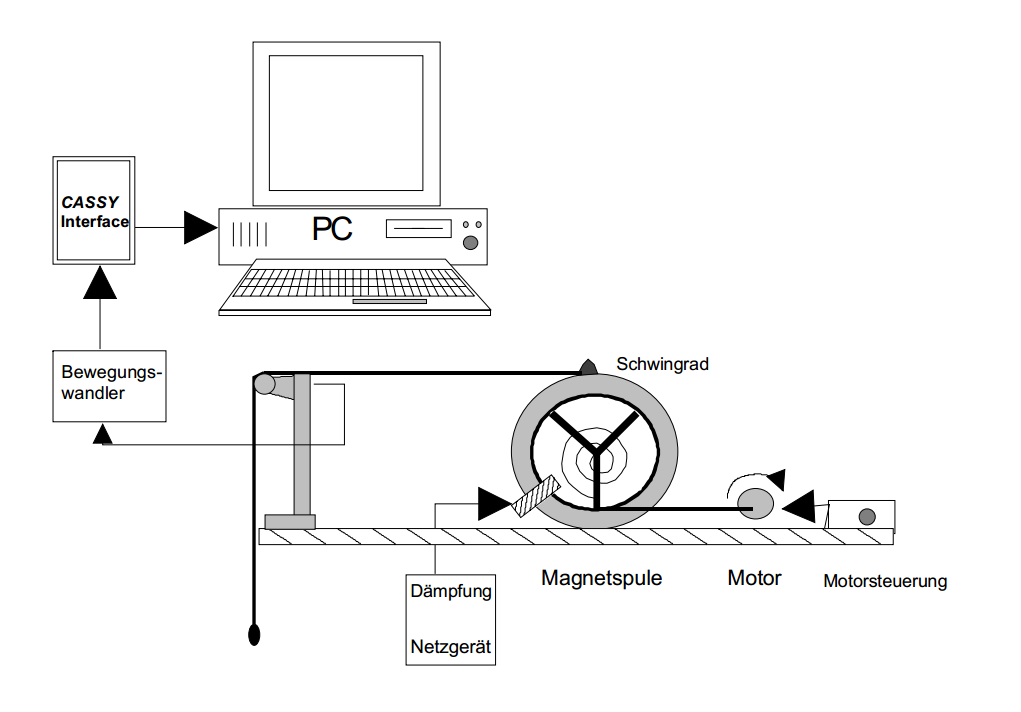
\includegraphics[width=9cm]{aufbau.png}
  \caption{Versuchsaufbau}
\end{wrapfigure}
Der Aufbau besteht aus einem horizontal gelagertem Rad an das eine Spiralfeder
monitiert ist, so dass es um die Ruhelage frei schwingen kann. An die
Spiralfeder ist ein Motor gekoppelt, der den Ruhepunkt in eine sinusförmige
Schwingung mit einstellbarer Frequenz versetzt. Von einer Wirbelstrombremse
kann eine geschwindigkeitsabhängige Dämpfung variabler Stärke erzeugt werden.

Das Rad ist mit einem Faden verbunden, der über ein Messrad (Rotationskodierer)
läuft und am anderen Ende mit einem geringen Gewicht beschwert ist. Des Messrad
ist an einen Bewegungswandler angeschlossen, der die Geschwindigkeit des Rades
in eine Spannung umsetzt, die mittels eines A/D-Wandlers vom angeschlossenen PC
gemessen wird. Die Software CASSY-Lab nimmt die Messdaten auf.

Zur Durchführung der ersten Aufgabe haben wir den Motor nicht benutzt. Wir
haben die Wirbelstrombremse auf die Stufen 1, 2 und 3 eingestellt, das Rad
ausgelenkt und dafür jeweils die Zeit/Geschwindigkeitskurve aufgenommen.

Für die Aufgaben 2, 3 und 4 haben wir die Dämpfungsstufe 2 gewählt und jeweils
Zeit/Geschwindigkeitskurven für verschiedene Motorfrequenzen direkt am PC
ausgewertet. Die Kurven in der Nähe der Resonanz und im Resonanzfall haben wir
direkt ausgedruckt.

\section{Auswertung}
\subsection{Aufgabe 1}
% TODO
Da wir leider keinen logarithmischen Plot direkt aus CASSY-Lab erstellt haben,
mussten wir hier zu einer anderen Methode greifen.

Zuerst haben wir zwei Maxima gesucht um aus der Zeitdifferenz und der Anzahl
der Perioden die Schwingungsfrequenz $\omega$ zu bestimmen.

Dann haben die Amplituden der einzelnen Maxima abgemessen. Wegen des ungeraden
Maßstabes des Papiers (1 Volt entspricht $9{,}1$ cm), haben wir diese in
Zentimetern abgemessen. Die Einheit ist für die Bestimmung der Konstanten
sowieso nicht relevant. Diese haben wir dann logarithmisch gegen die Zeit
aufgetragen, die sich rechnerisch aus der Frequenz ergibt.


\subsection{Aufgabe 2}
Wir haben jeweils für verschiedene Erregerfrequenzen die
Zeit/Geschwindigkeitskurven aufgenommen. Die Frequenz bestimmen wir, indem wir
zwei die Zeiten zweier Maxima ($t_1$, $t_2$) bestimmen und die Anzahl der
Perioden ($n$) abzählen. Der Fehler der Zeiten ist dabei $\Delta t =
\SI{0.1}{s}$, da wir mit dieser Auflösung messen. Die Anzahl der Maxima ist
keine fehlerbehaftete Größe.

Wir erhalten die Frequenz
\begin{equation}
  \Omega = \frac{2 \pi}{T} = 2 \pi \frac{n}{t_2 - t_1}
\end{equation}

mit dem Fehler
\begin{align}
  \Delta \Omega &= \sqrt{
    \del{\partial{\Omega}{t_2}}^2 \Delta t_2^2 +
    \del{\partial{\Omega}{t_2}}^2 \Delta t_1^2 +
  } \\
  &= \sqrt{
    \del{-\frac{2 \pi n}{(t_2 - t_1)^2}}^2 +
    \del{\frac{2 \pi n}{(t_2 - t_1)^2}}^2
  } \Delta t \\
  &= \sqrt{2} \frac{2 \pi n}{(t_2 - t_1)^2} \Delta t
\end{align}

Die Amplitude haben wir in Volt gemessen. Für die Ermittlung der Konstanten
spielt dies jedoch keine Rolle, da der Umrechnungsfaktor sich herrauskürzt.

Die Phasenverschiebung haben wir geschätzt. Man kann erkennen, ob die Bewegung
des Erregers und des Rades gleich- oder gegenläufig ist oder irgendwelche Werte
grob dazwischen annimmt. Deswegen nehmen wir den großen Fehler $\frac{\pi}{2}$ an.

Die in unbekannten Einheiten eingestellte Kreisfrequenz $\Omega$ tragen wir
zusammen mit der berechneten Kreisfrequenz (ebenfalls $\Omega$), der Amplitude
(gemessen in Volt) und der geschätzten Phasenverschiebung $\phi_0$ in der
folgenden Messwerttabelle ein.

\begin{tabular}{r|r|r|r}
  $\Omega$ [?] & $\Omega$ [1/s] & $A_0$ [V] & $\phi_0$ [rad] \\
  \hline
  208 & $\num{4.504+-0.024}$ & $\num{0.096+-0.002}$ & $\num{-3.1+-1.6}$ \\
  200 & $\num{3.973+-0.022}$ & $\num{0.125+-0.002}$ & $\num{-3.1+-1.6}$ \\
  180 & $\num{3.898+-0.020}$ & $\num{0.147+-0.002}$ & $\num{-3.1+-1.6}$ \\
  160 & $\num{3.842+-0.020}$ & $\num{0.183+-0.004}$ & $\num{-3.1+-1.6}$ \\
  130 & $\num{3.765+-0.020}$ & $\num{0.269+-0.008}$ & $\num{-1.6+-1.6}$ \\
  110 & $\num{3.695+-0.016}$ & $\num{0.358+-0.008}$ & $\num{-1.6+-1.6}$ \\
  100 & $\num{4.665+-0.033}$ & $\num{0.388+-0.008}$ & $\num{-1.6+-1.6}$ \\
  90  & $\num{3.695+-0.020}$ & $\num{0.430+-0.004}$ & $\num{-1.6+-1.6}$ \\
  70  & $\num{5.347+-0.040}$ & $\num{0.388+-0.006}$ & $\num{-1.6+-1.6}$ \\
  30  & $\num{3.515+-0.017}$ & $\num{0.209+-0.004}$ & $\num{ 0.0+-1.6}$ \\
  10  & $\num{3.442+-0.017}$ & $\num{0.152+-0.002}$ & $\num{ 0.0+-1.6}$ \\
\end{tabular}

\vspace{1cm}

In Plot \textit{Resonanzkurve} haben wir die Amplitude $A_0$ über die Frequenz
$\Omega$ aufgetragen.

Wir fitten diese Daten gegen Gleichung \ref{eq:amp}, die den theoretischen
Zusammenhang zwischen Ampltitude und Erregerfrequenz angibt.

Dabei sind vier Ausreißer zu erkennen, die wir gestrichelt eingezeichnet haben
und nicht für den Fit verwenden. Sie lassen sich dadurch erklären, dass wir
beim Ablesen der Zeiten oder der Anzahl der Amplituden Fehler gemacht haben.
Auch in der Messwerttabelle kann man an diesen Stellen unplausible Werte für
$\Omega$ erkennen.

Die Werte für die Dämpfungskonstante $\delta$ und die Eigenfrequenz $\omega_0$
können wir aus dem Plot ablesen.  Die angegebenen Fehler sind die jeweiligen
Fehler die bei der Methode der kleinsten Quadrate anfallen
(Standardabweichung). Das Endergebnis lautet

\begin{align}
  \omega_0 &= \SI{3,675+-0.006}{s^{-1}} \\
  \delta &= \SI{0.083+-0.005}{s^{-1}}
\end{align}

\subsection{Aufgabe 3}
Aus der Messwerttabelle kann man erkennen, dass die Phasenverschiebung
frequenzabhängig ist. Sie nimmt Werte zwischen $0$ (Frequenzen unterhalb der
Resonanzfrequenz) und $-\pi$ (Frequenzen oberhalb der Resonanzfrequenz) an. Ist
die Frequenz in der Nähe der Resonanzfrequenz, tritt ungefähr eine
Phasenverschiebung von $-\frac{\pi}{2}$ auf.

Die ermittelten Werte stützen dabei den Zusammenhang in Gleichung \ref{eq:tan}.
Genauso möglich wäre aber ein linearer Verlauf. Die Daten sind zu ungenau um
exaktere Aussagen zu treffen.

\subsection{Aufgabe 4}
Anhand der Grafik des Einschwingvorgangs im Resonanzfall kann man sehen, dass
die Maximalamplituden des ungefähr einem exponentiellen Verlauf
$A_\text{max}(t) \propto 1 - e^{- a t}$ folgen.

Wenn man die Bewegungsgleichung für den Einschwingvorgang
(\ref{eq:ein}) betrachtet, sieht man, dass im Resonanzfall $\omega_0 = \Omega$
die Kosinusterme die selbe Frequenz haben. Die Phasenverschiebung $\phi$ ist
dabei $-\frac{\pi}{2}$, somit erhält man

\begin{equation}
  x(t) = A_S \del{1 - e^{-\delta t}} \sin \omega_0 t
\end{equation}

Dies entspricht exakt der Beobachtung.

In der nähe der Resonanz schwingen die Maximalamplituden mit einer Frequenz,
die wesentlich größer ist als die Erreger- oder die Resonanzfrequenz.

Nehmen wir erneut Gleichung \ref{eq:ein} und nehmen aufgrund der Nähe zur
Resonanz näherungsweise eine Phasenverschiebung von $-\frac{\pi}{2}$ an,
erhalten wir
\begin{align}
  x(t) &= A_s \del{\sin(\Omega t) - e^{-\delta t} \cos(\omega_0 t)} \\
       &= A_s \del{\sin(\Omega t) + \cos(\omega_0 t) - (e^{-\delta t} - 1) \cos(\omega_0 t)}
\end{align}

Für kleine Zeiten $t$ verschwindet der letzte Term, so dass am Anfang des
Einschwingvorgangs der folgende Term dominiert:
\begin{equation}
  x(t) \approx A_s \del{\sin(\Omega t) + \cos(\omega_0 t)}
\end{equation}

Per Additionstheorem erhalten wir
\begin{equation}
  x(t) \approx 2 A_s \sin\del{\frac{\Omega - \omega_0}{2} + \frac{\pi}{4}}
  \sin\del{\frac{\Omega + \omega_0}{2} + \frac{\pi}{4}}
\end{equation}

Der erste Term schwingt mit der großen Frequenz $\frac{\Omega - \omega_0}{2}$.
Hier tritt also offensichtlich zu Anfang des Einschwingvorgangs eine Schwebung
mit dieser großen Frequenz auf.

Dies entspricht ebenfalls genau der Beobachtung.

\section{Zusammenfassung und Diskussion}
Wir haben mithilfe des Pohlschen Rades ungetriebene und getriebene harmonische
Oszillationen mit ihren Resonanzen untersucht. Wir konnten mithilfe der
Resonanzkurve die Eigenfrequenz und Dämpfungskonstante des Pohlschen Rades sehr
genau bestimmen:

\begin{align}
  \omega_0 &= \SI{3,675+-0.006}{s^{-1}} \\
  \delta &= \SI{0.083+-0.005}{s^{-1}}
\end{align}

Auch konnten wir den Verlauf der Amplitudenmodulation beim Einschwingvorgang
anhand der theoretischen Überlegungen erklären.

Die Phasenverschiebung wurde nur visuell geschätzt. Mit einem veränderten
Aufbau des Experiments hätten wir die treibende Kraft messen können, zum
Beispiel mit einem zweiten Messrad und so eine bessere Übereinstimmung der
Phasenverschiebung mit den theoretischen Werten zu zeigen.

Beim Ablesen der Werte vom Bildschirm sind offenbar einige Fehler aufgetreten,
die vermeidbar gewesen wären.  Wenn wir die Daten ausgedruckt hätten oder der
Messcomputer über einen Internetzugang verfügt hätte, hätten wir diese Fehler
korrigieren können.

Da wir die Ausreißer jedoch identifizieren konnten, hat dies die Resultate
nicht beeinflusst.

\newpage
\label{plot:damp}
\begin{landscape}
  % gnuplot ./plot-daempfung.gnuplot
  \input{plot-daempfung.tex}
\end{landscape}

\newpage
\label{plot:amp}
\begin{landscape}
  % gnuplot ./plot.gnuplot
  \input{plot.tex}
\end{landscape}


\end{document}
